\documentclass[english]{upeeei}
\usepackage[latin9]{inputenc}
\setcounter{secnumdepth}{3}
\setcounter{tocdepth}{3}
\usepackage[active]{srcltx}
\usepackage{units}
\usepackage{parskip}
\usepackage{graphicx}
\usepackage{subfigure} 
\usepackage{url}  
%\usepackage{stfloats}  
\usepackage{amsmath}   
\usepackage{array}
\usepackage{caption}
\usepackage{afterpage}
\usepackage{textcomp}
\usepackage{lscape}
\usepackage{stfloats}
\usepackage{hyphenat}
\usepackage{makeidx}
\usepackage{amssymb}
%\usepackage{underscore}
\fnbelowfloat
\usepackage{times}
\usepackage{multirow}
%\usepackage{float}
\usepackage{circuitikz}
\usepackage[backend=bibtex,bibstyle=ieee,citestyle=numeric-comp]{biblatex}
\addbibresource{Proposal_Part1.bib}
\usepackage{pgfplots}
%\usepackage{arydshln}
\pgfplotsset{width=7cm,compat=1.5.1}
\renewcommand*{\bibfont}{\small}

\newcolumntype{L}[1]{>{\raggedright\let\newline\\\arraybackslash\hspace{0pt}}m{#1}}
\newcolumntype{C}[1]{>{\centering\let\newline\\\arraybackslash\hspace{0pt}}m{#1}}
\newcolumntype{R}[1]{>{\raggedleft\let\newline\\\arraybackslash\hspace{0pt}}m{#1}}

\newcommand\ddfrac[2]{\frac{\displaystyle #1}{\displaystyle #2}}
\pgfplotsset{compat=1.14}

\makeatletter

%%%%%%%%%%%%%%%%%%%%%%%%%%%%%% LyX specific LaTeX commands.
\providecommand{\LyX}{L\kern-.1667em\lower.25em\hbox{Y}\kern-.125emX\@}
%% Because html converters don't know tabularnewline
\providecommand{\tabularnewline}{\\}

\@ifundefined{showcaptionsetup}{}{%
 \PassOptionsToPackage{caption=false}{subfig}}
\usepackage{subfig}
\makeatother

\usepackage{babel}

\begin{document}
%%% UP EEEI undergraduate project template
%% v0.1 by Louis P. Alarcon 11/22/2011
%%
%% LyX template - use with the following files:
%% 	uct10_new.clo, uct11_new.clo, uct12_new.clo, upeeei.cls, upeeei.layout
%%
%% Place project title here
\title{Autonomous 3D Indoor Mapping Using Unmanned Aerial Vehicles} 

%%
%% Author information

\author{
%% Use \vspace to separate each member
%% Put your names here in alphabetical order
\\Louie Isaniel Cachola Henson \\ 2014-30227 \\ \emph{B.S. Computer Engineering}
}

%%
%% Month and year of submission/graduation
\degreeyear{2021} 
\degreesemester{January} 

% Put your advisers here:
\chair{Professor Charleston Dale Ambatali
\\
Roxanne P. De Leon, ECE, MTM
} 
%\othermembers{John Richard Ereso Hizon\\ 
%Joel Joseph Sarco Marciano, Jr.} 
\numberofmembers{1} 

\field{Electrical/Computer/Electronics and Communications Engineering} 
\campus{Diliman} 

\maketitle
% \approvalpage 
% \copyrightpage 
\begin{abstract} 

%Your abstract goes here...


Multirotor unmanned aerial vehicles (or drones as they are more commonly known) are quick and versatile, often 
proving to be a great asset for various purposes. It is because of this that a host of flight controllers
have been developed using open-source technology

The project aims to provide search and rescue
personnel a means to efficiently map out an area, lending them a smart tool for better planning and risk assessment.
The goal of this project is to develop a drone that can autonomously provide the user with an
accurate 3D map of indoor spaces. This would require a robust flight controller capable of
accurate simultaneous localization and mapping (SLAM) and efficient 3D navigation and exploration. Performance of the UAV
will be assessed in terms of exploration speed and mapping precision.

\end{abstract}

\begin{frontmatter}
\setlength{\parskip}{0pt}
\tableofcontents
%\listoftables
\listoffigures
\end{frontmatter}
\def\MASTERDOC{true}

\chapter{Introduction}
Unmanned aerial vehicles continue to be integrated into increasingly diverse environments and
fields. From photography and cinematography, all the way to military applications. Similarly, mapping drones have found uses
in fields such as archaeology and architecture, all the way to disaster risk reduction and management. They are especially
useful for reducing the amount of risk that personnel experience by flying to places that pose a significant hazard to 
the personnel \cite{ICNSC2010}. The problem, however, lies in mapping out indoor spaces, especially those where flight may
be restricted by narrow paths and obstacles. Maneuvering through small spaces can prove to be difficult even for experienced
pilots and could lead to a crash. Crashes are costly as the worst of them could require the replacement of the entire UAV.
Furthermore, UAV flight times are restricted by their battery capacity. Hence, in order to maximize the use of the UAV, there
must be a way to explore unknown spaces efficiently.
One possible solution to this is the development of a mapping UAV with autonomous navigation and exploration functions. By
limiting the amount of ways that the pilot can influence the actual movement, the risk of human error is limited \cite{AutoFunc}.
Furthermore, we can employ various algorithms for more efficient exploration, as will be explored further in this document. 
\newline
\newline
The development of a flight controller 
system capable of autonomous 3D indoor mapping can be divided into the development of several components; the flight 
controller board, the SLAM (simultaneous localization and mapping) algorithm, and the autonomous navigation function.
\section{Flight Controller Design}
The flight controller is, as its name suggests, the central device that controls how the UAV moves and reacts to certain
stimuli. The flight controller contains multiple sensors including (but not limited to) a gyroscope, accelerometer, and
barometer. These sensors allow the flight controller to get a sense of its orientation in 3D space. The flight controller 
will also be responsible for communicating with a base station and processing commands correctly. In order to make the
UAV easy to mass produce and more affordable, production cost was prioritized while designing the flight controller.
Several methods for designing the flight controller were found but one was seen to be the most cost-effective and
flexible solution. Establishing a well functioning flight controller is important as it is essentially the cornerstone of the
UAV and will influence work on both the autonomous navigation functions as well as the simultaneous localization and
mapping (SLAM) functions.
\section{Simultaneous Localization and Mapping}
Simultaneous localization and mapping (SLAM) is the process where a machine maps out its immediate environment and gets
a sense of where it is in that environment. This is especially useful for autonomous exploration as it allows the UAV to
formulate an obstacle-free trajectory to its target. Mapping often makes use of a lidar sensor
\cite{Dowling2018} or one or more cameras\cite{OrbSlam2} depending on the level of accuracy and speed that is required. 
\section{Autonomous Navigation}
Autonomous navigation is the process where a machine navigates to a target location while avoiding obstacles. This is
often used in tandem with SLAM and path finding algorithms such as Dijkstra's algorithm or even neural networks 
\cite{Dowling2018}. Methods of navigation include global and local navigation however Dowling et al. note that the
best results can be found by combining the two \cite{Dowling2018}.

\chapter{Review of Related Work}
\section{Flight Controller Board Design}
As building a flight controller from scratch would prove to be akin to reinventing the wheel, a premade flight controller
will be used as a base that this project will build upon. The base flight controller will be responsible for communicating
with the electronic speed controllers (ESCs) and controlling the motors on a more basic level \cite{MultiwiiFC}. 
The corresponding diagram for the system is represented by figure \ref{fig:base_FC_diagram}. The flight controller makes 
use of a microcontroller that is connected to an inertial
\begin{figure}[h]
    \centering
    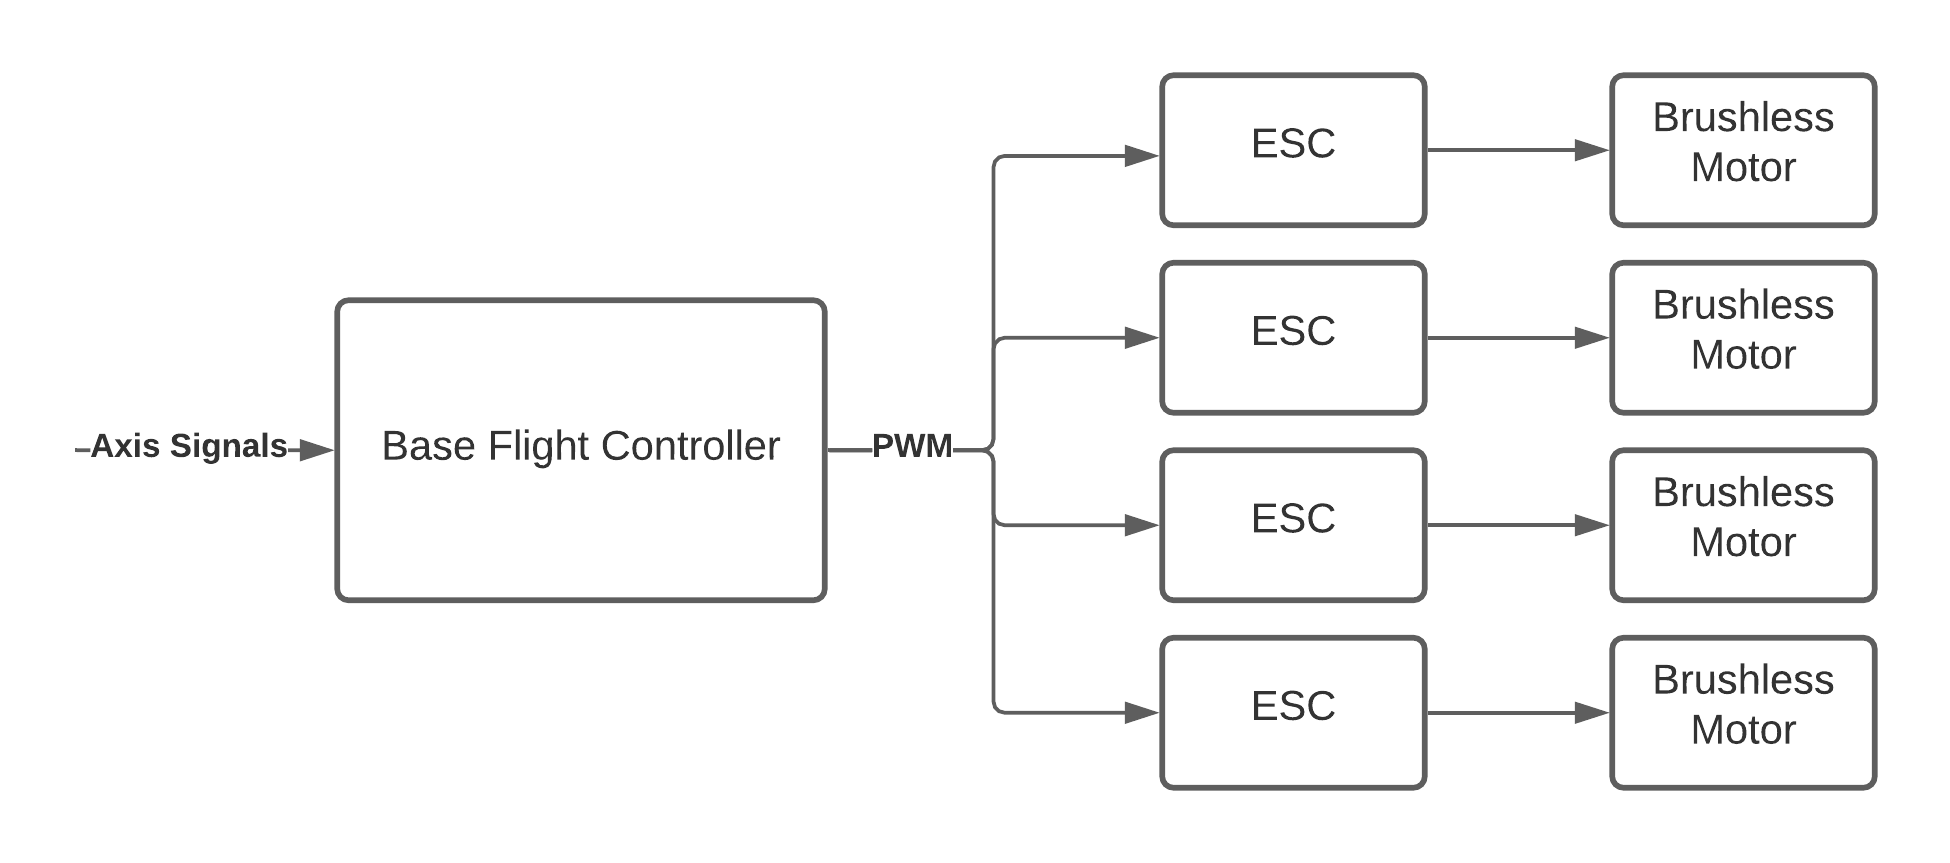
\includegraphics[scale=0.5]{images/base_FC_diagram.png}
    \caption{Diagram of base flight controller connected to ESCs and motors}
    \label{fig:base_FC_diagram}
\end{figure}
measurement unit (IMU). The IMU includes an accelerometer and gyroscope that allow the flight controller to discern its 
orientation in 3-dimensional space. Based on these readings, the flight controller will update the ESCs with the proper
outputs. Based on figure \ref{fig:base_FC_diagram}, we will essentially be treating the base flight controller as a black
box. The inputs would be a PPM signal containing the throttle, yaw, pitch, and roll signals \cite{MultiwiiFC}.
The Pixhawk, another family of flight controllers, make use of MAVLink (Micro Air Vehicle Communication Protocol) to 
deliver the necessary signals into the flight controller. MAVLink makes use of a UART
connection to send instructions to the flight controller. 
S. Al-Kadhim demonstrates how to makes use of a Raspberry Pi to communicate with the Pixhawk \cite{RPiMavlink2019}. This 
allows them to interface with the UAV in a more sophisticated manner and make use of the computer's
higher processing power. Other known applications of onboard computers on UAVs is the application of neural networks for
autonomous flight \cite{Redtail2017}. Meanwhile, Dowling et al. use a Raspberry Pi coupled with a lidar sensor to allow the UAV
to autonomously navigate and map out its surroundings on a 2D plane \cite{Dowling2018}. This is shown in figure 
\ref{fig:FC_system_diagram}.
\begin{figure}[h]
    \centering
    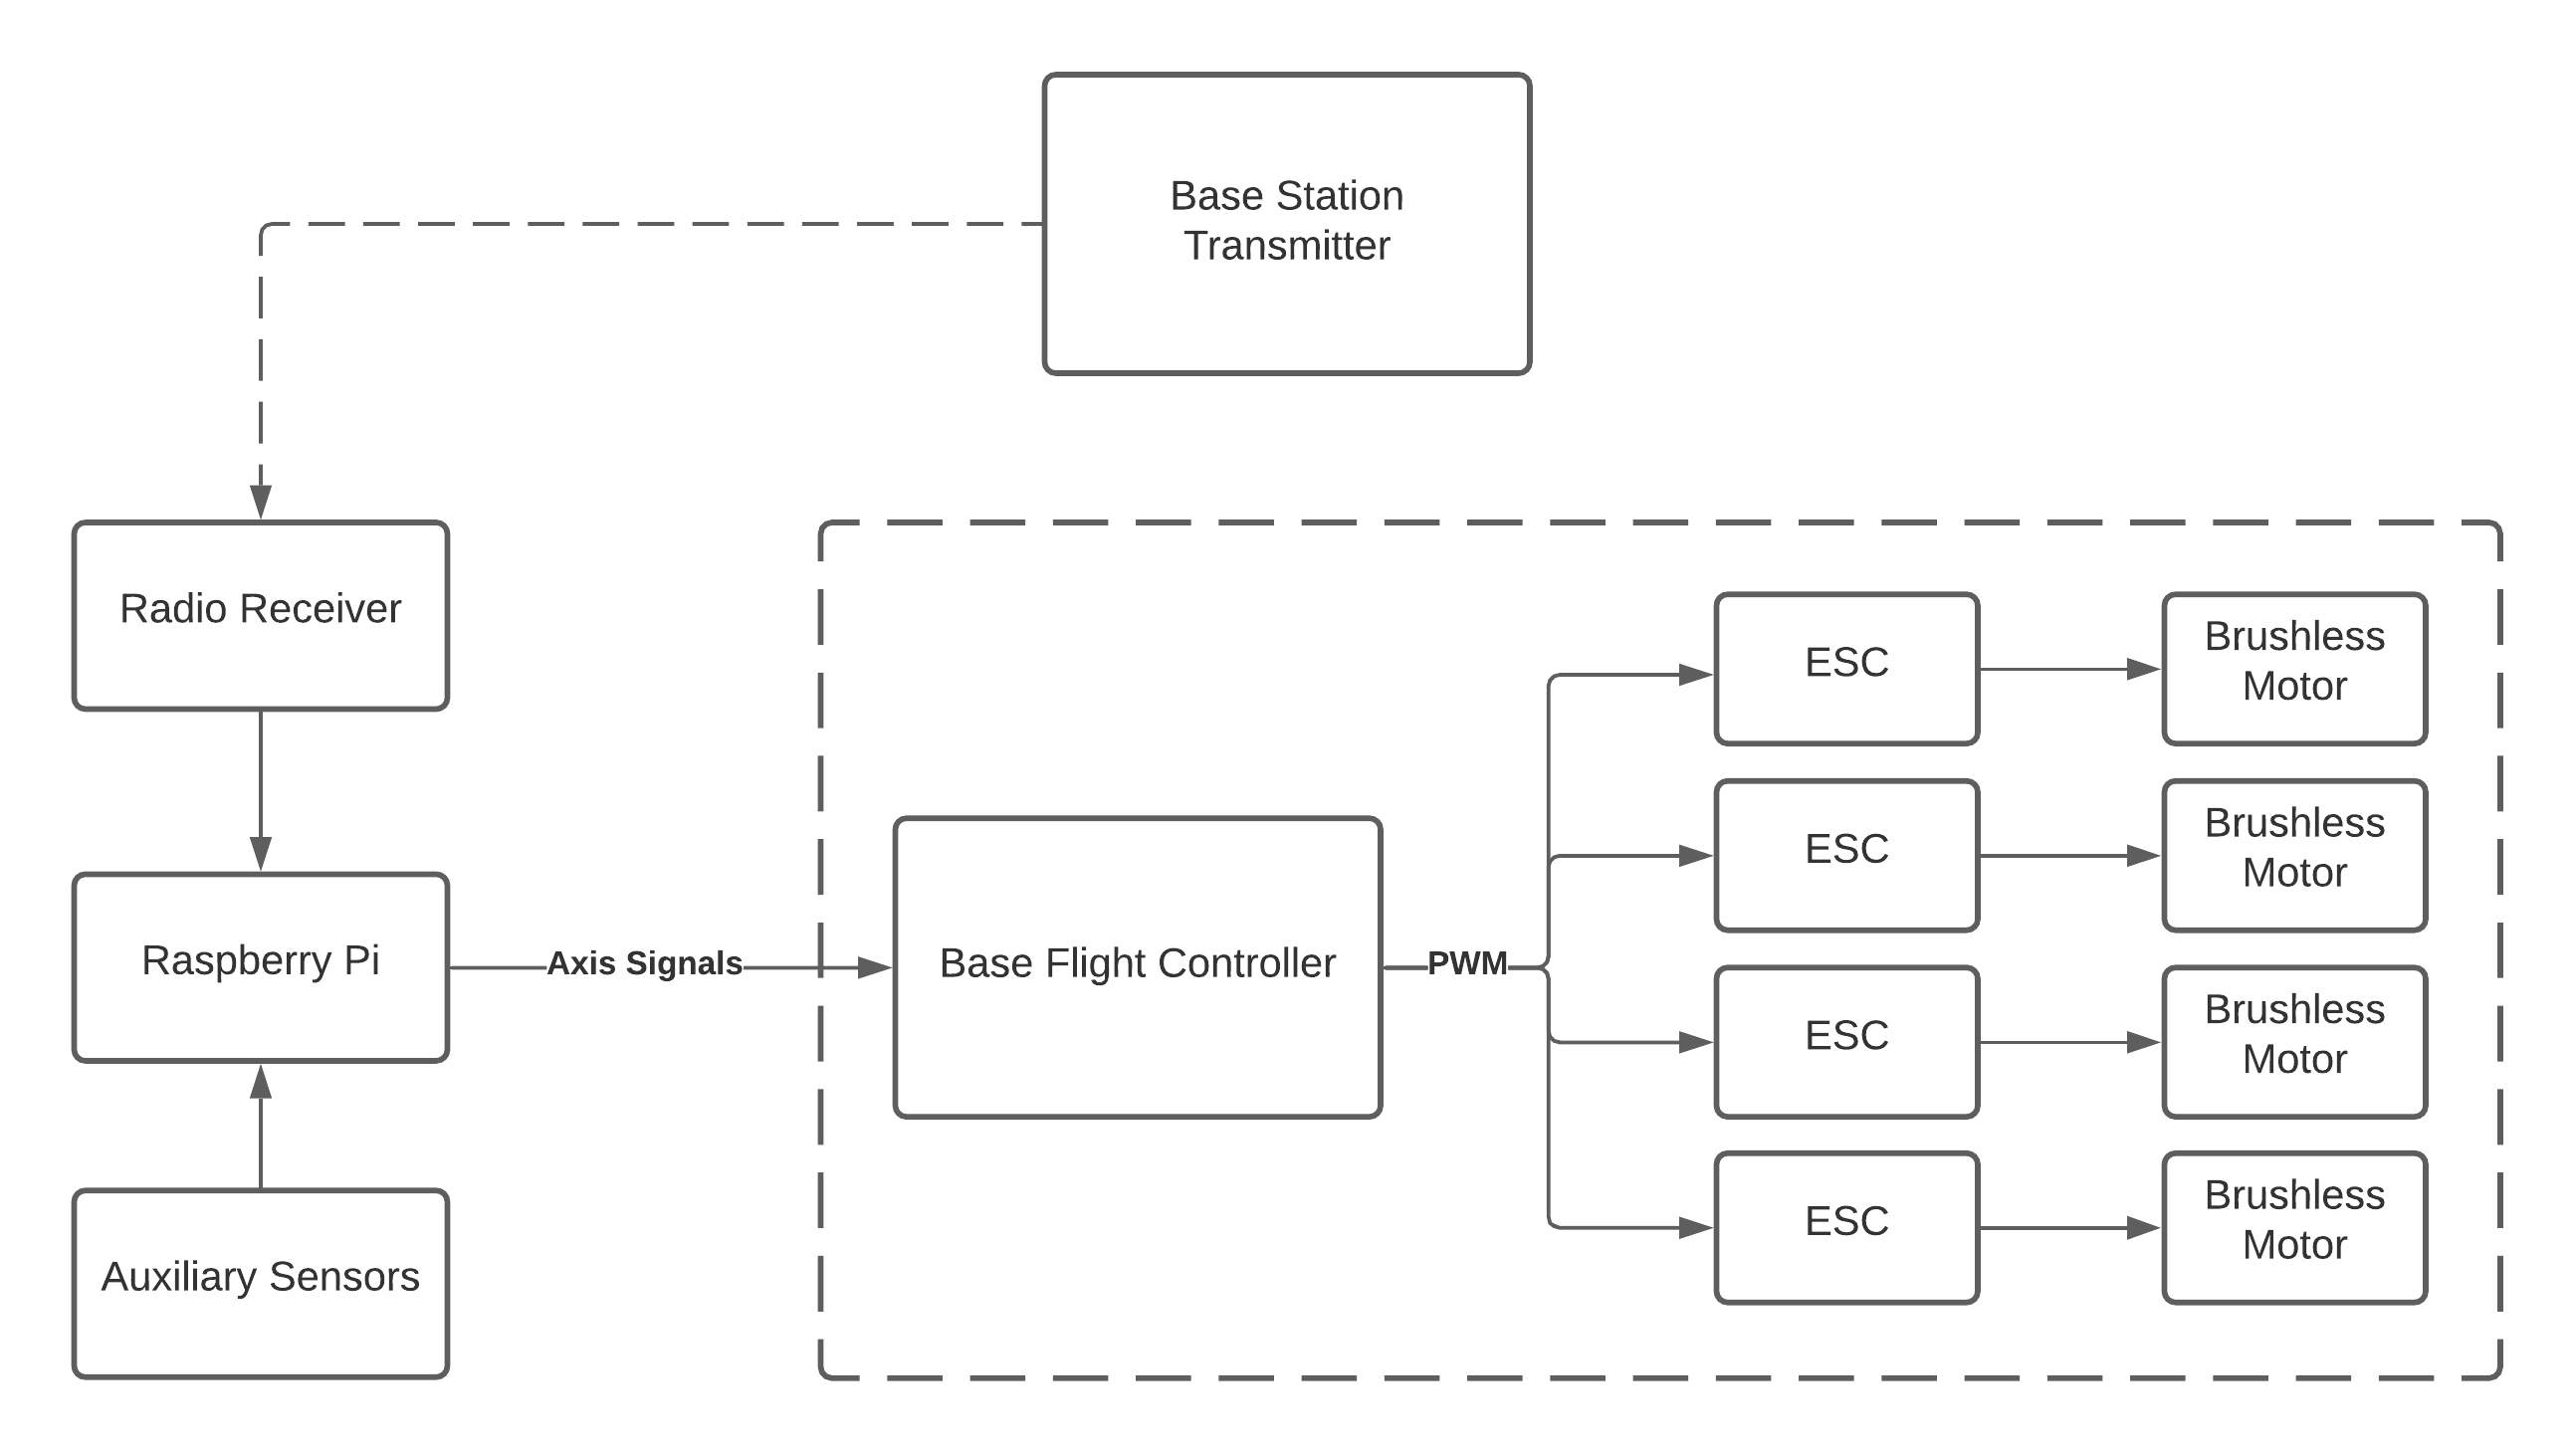
\includegraphics[scale=0.5]{images/fc_with_rpi.png}
    \caption{Diagram of flight controller system with raspberry pi}
    \label{fig:FC_system_diagram}
\end{figure}
The base flight controller itself is akin to a PID controller. The firmware allows us to manually tune the PID values depending 
on the user's preference. Saengphet et al. demonstrate a more robust way of tuning the PID values as compared to the
more traditional heuristic methods. It involves conducting piloted test flights to see how the UAV responds to certain stimuli
\cite{Tuning2017}.
\section{Simultaneous Localization and Mapping}
An open-source SLAM API was proven to be functional by Mur-Artal et al\cite{OrbSlam1}. The API makes use of a monocular camera as an
input device and is able to reconstruct both indoor and outdoor environments in real time. This SLAM system was developed
with ground based robots and cars in mind. It essentially works by selecting a number of points of interest in one frame
\begin{figure}[h]
    \centering
    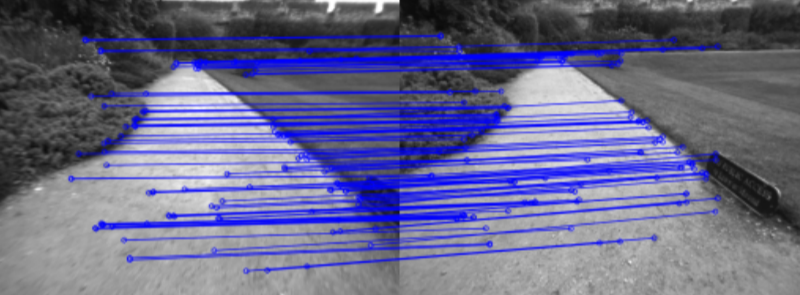
\includegraphics[scale=0.5]{images/orbslam1_feat_tracking.PNG}
    \caption{Frame by frame point matching by ORB SLAM 1\cite{OrbSlam1}}
    \label{fig:orbslam1_tracking}
\end{figure}
of the video then matching these points to similar points of interest in the next frame. It then takes the difference in
position of these point of interest and calculates depth from there.
\newline
\newline 
The authors then further improved the accuracy in
a second iteration\cite{OrbSlam2}. Here, they expanded the input to stereo cameras and depth cameras as these seemed to provide much more
accurate results. The authors found that using only a monocular camera was prone to failures as more rotations were used
in the machine's exploration. They also found that using a depth camera or multiple cameras (as in the stereo camera) significantly
improved the accuracy of depth perception. 
\begin{figure}[h]
    \centering
    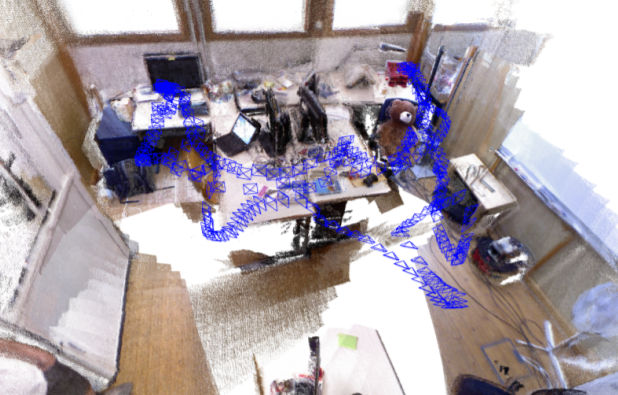
\includegraphics[scale=0.5]{images/orbslam2_recon.PNG}
    \caption{3D reconstruction of a room by ORB SLAM 2 using a depth camera. Marked in blue is the trajectory of the camera\cite{OrbSlam2}}
    \label{fig:orbslam2_recon}
\end{figure}
Another aspect that the authors improved upon is the fact that this version
was developed to be an out-of-the-box SLAM solution. As a result, this version provides more support for varying systems
and is much easier to use as compared to the previous version. However this version does have its lapses where processing
power is concerned. Due to the heavy operations being performed, it would struggle to perform even on a Raspberry Pi 4. 
\newline
\newline
Looking for a lightweight SLAM solution, FastSLAM 2.0 presents a SLAM system for low-power embedded architectures \cite{FastSlam2},
which would be more ideal for the purposes of this project. The authors used a 320x300 resolution camera connected to a
Raspberry Pi 2B. While the system was able to function within the low-power specifications, it suffers in terms of
\begin{figure}[h]
    \centering
    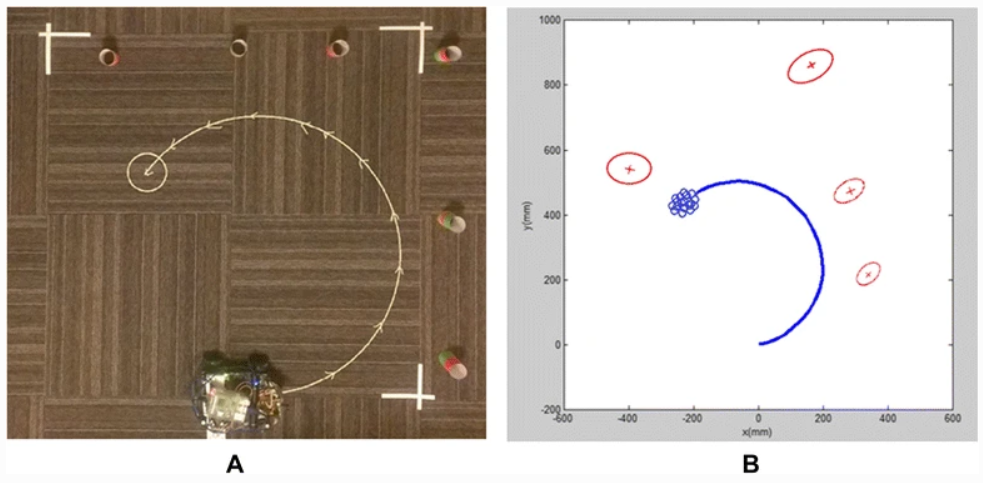
\includegraphics[scale=0.5]{images/fastslam2.PNG}
    \caption{Top view of a robot navigating through a corner (A) and the corresponding Fast SLAM map (B). The robot's trajectory
    is denoted by the blue line while obstacles are denoted by the red figures.\cite{FastSlam2}}
    \label{fig:fastslam_results}
\end{figure}
accuracy. The system was significantly less accurate than the SLAM systems discussed previously \cite{OrbSlam1,OrbSlam2}. 
While there were no direct measured comparisons between ORB SLAM 2 and FastSLAM2.0, FastSLAM2.0 was only able to detect 
75\% of obstacles presented to it. As seen in figure \ref{fig:fastslam_results}, while navigating a corner of obstacles,
the robot failed to detect 2 of the 6 obstacles. 
The authors claim that this was due to the low resolution of the camera used and that accuracy can be further improved
by using an encoder with a higher resolution. 
\newline
\newline
Finally, Forster et al. present a lightweight but accurate solution for
localization and mapping with Semi-direct Visual Odometry (SVO) \cite{SVO2017}. Primarily developed for use with
UAVs and monocular cameras, SVO boasts a reduction in CPU usage of up to 79.45\% compared to ORB SLAM 1. 
SVO is also up to 11.8 times faster while maintaining an accuracy that is 13.5 times better than that of ORB SLAM 1. 
A summary of the comparison between monocular ORB SLAM 1 and SVO may be seen in figure \ref{fig:SVO_VS_ORB}. SVO is faster
because it needs to process less data. While ORB SLAM 1 and 2 extract features and descriptors from every frame, SVO only
does this for a few key frames. 
\begin{figure}[h]
    \centering
    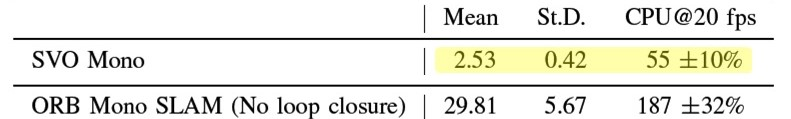
\includegraphics[scale=0.5]{images/SVO_CPU_time.jpg}
    \caption{Comparison of and ORB SLAM 1 and SVO\cite{SVO2017}}
    \label{fig:SVO_VS_ORB}
\end{figure}
\section{Autonomous Navigation}
Autonomous navigation consists of two methods; global and local. Global navigation methods involve planning out the general
trajectory of the robot without taking into account the local movement restriction of the robot. This entails planning out
the overall path that the robot will take when reaching its goal. By contrast, local navigation methods involve planning
the trajectory of the robot around its direct environment. This involves more minute movements and obstacle avoidance. 
According to Dowling et al., the best navigation results have been obtained by combining both of these methods\cite{Dowling2018}. The
navigation system used by Dowling et al. mimics navigation systems used by ground based robots and adapts them to suit
UAVs flying at a fixed height. Their system simulates all possible trajectories that the UAV can take and assigns a cost
to each one. The UAV then takes the path with the smallest cost. While this method functions well for 2D mapping and
navigation, this would be lacking for this project as we would need to navigate in 3D. Luckily, Zhou et al. present a method 
for performing fast UAV exploration in complex environments (FUEL)\cite{Fuel2020}. It starts similarly by finding the most optimal
global trajectory that is available to the UAV. It then continually recalculates as more and more regions are explored.
FUEL is based on the frontier method of navigation where the UAV looks for the nearest unexplored region. The authors also
introduce a frontier information structure (FIS) that contains information on the environment. The structure is then updated
continuously and allows for high frequency planning. Based on the FIS, the system then generates a heirarchy of motions
in three steps (course to fine). The heirarchical planner finds efficient global paths, selects a local set of optimal
viewpoints, and from there, generates the best trajectory based on the minimum time. Figure \ref{fig:fueltest} shows a test
run by using the classical frontier method as a benchmark. As we can see, the FUEL method is more efficient, generating the
shorter path.
\begin{figure}[h]
    \centering
    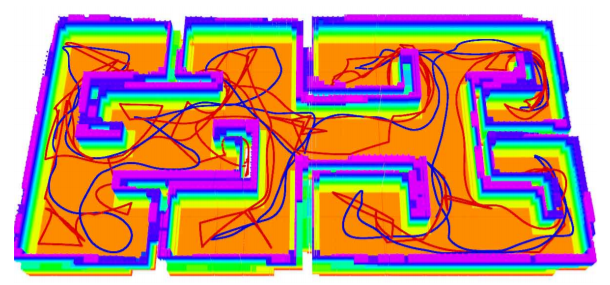
\includegraphics[scale=0.5]{images/fueltest.PNG}
    \caption{Path generated by frontier method (red) and FUEL method (blue)\cite{Fuel2020}}
    \label{fig:fueltest}
\end{figure}
Alternatively, Xu et al. present a 
different method of navigation that deviates from the frontier method and instead adopts a method based on incremental sampling
and a probabilistic roadmap \cite{ProbNav}. In this method, nodes are incrementally added to the explored regions to
generate the best viewpoints for the camera system. These viewpoints are those that provide the system with the most data
points, thereby mapping the most amount of regions in the least time. The probabilistic roadmap allows for rapid searching
of alternative global and local paths that the UAV can take. However the authors found that the system was not able to
locate all obstacles 100\% of the time, raising concerns with regards to the safety of the UAV while navigating. The authors
compared the method's performance to that of the frontier method. The results may be seen in figure \ref{fig:deptest}. After 10
minutes of exploration, the probabilistic roadmap method was able to explore more regions than the frontier method.
\begin{figure}[h]
    \centering
    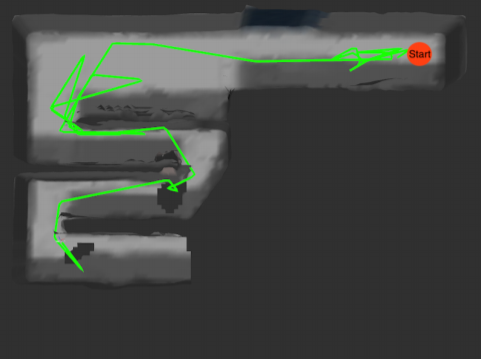
\includegraphics[scale=0.5]{images/dep_frontier.PNG}
    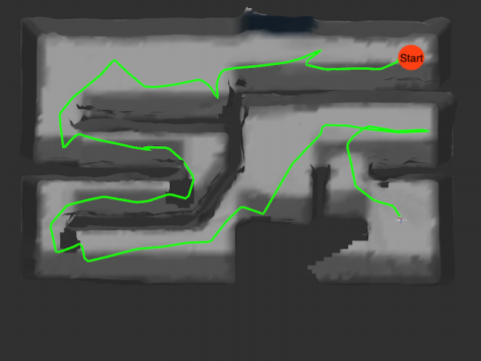
\includegraphics[scale=0.5]{images/dep_dep.PNG}
    \caption{Regions explored and path generated by frontier method (left) vs proposed probabilistic roadmap method (right) after
    running for 10 minutes. \cite{ProbNav}}
    \label{fig:deptest}
\end{figure}
\chapter{Objectives}
This project aims to develop a low-cost and lightweight UAV capable of autonomous 3D indoor mapping. Given an enclosed
indoor space, the UAV should be able to autonomously and completely explore and map out all enclosed regions while navigating at
a speed of at least 0.5m/s. 
During flight, the UAV should be able to transmit the mapped data to the base station so that the user has real-time feedback of
how the mission is progressing. On top of this, the UAV should also be able to function non-autonomously. The drone should be
able to be piloted manually through a pilot interfacing with the base station. 
\chapter{Preliminary Work}
\section{Flight Controller Design and Fabrication}
Cost, size, and weight were the primary deciding factors for the flight controller design. For the base flight
controller, the MultiWii was implemented as seen in figure \ref{fig:base_FC_diagram}. This allows for a much more flexible
and cost effective solution. The microcontroller used was the Arduino Pro Mini, which provides a small
footprint. It was then wired to send pwm signals to a 4-in-1 ESC board. A 4-in-1 ESC board was selected over
individual ESC modules because the board is lighter, smaller, and is less costly. Furthermore, less wiring will need to
be done, leading to easier mass production. The motors are 2400KV brushless motors suitable for 5 inch propellers.
For the inertial measurement unit, the MultiWii was connected to an MPU6050 via an I2C interface. The MPU6050 includes
both an accelerometer and a gyroscope. The arduino receives instructions from a Raspberry Pi 4. There are two
options for communication between the Raspberry Pi and the Arduino; single wire PPM and PWM over multiple wires. Both
methods were tested to find the method with the most stable signal. It was found that the signals gained from PWM over
multiple wires was noisy. PPM gave a much more consistent signal and so it was chosen as the mode of communication.
The Raspberry Pi will also be receiving data from a GY-87 module, which contains an accelerometer, gyroscope, barometer, 
and magnetometer which are all accessible via I2C protocol. This will aid the UAV with regards to SLAM and navigation. 
Aside from this, the Raspberry Pi is also connected to a GPS module which, while inoperable during indoor operations,
will prove to be essential during outdoor missions especially when locating the UAV. For communication, the flight controller 
employs a LoRa RA-02 module, which was chosen for its long range capabilities. The LoRa module will be communicating with a 
similar module connected to the base station. A diagram of the system may be seen in figure \ref{fig:final_FC_diagram}. 
\begin{figure}[h]
    \centering
    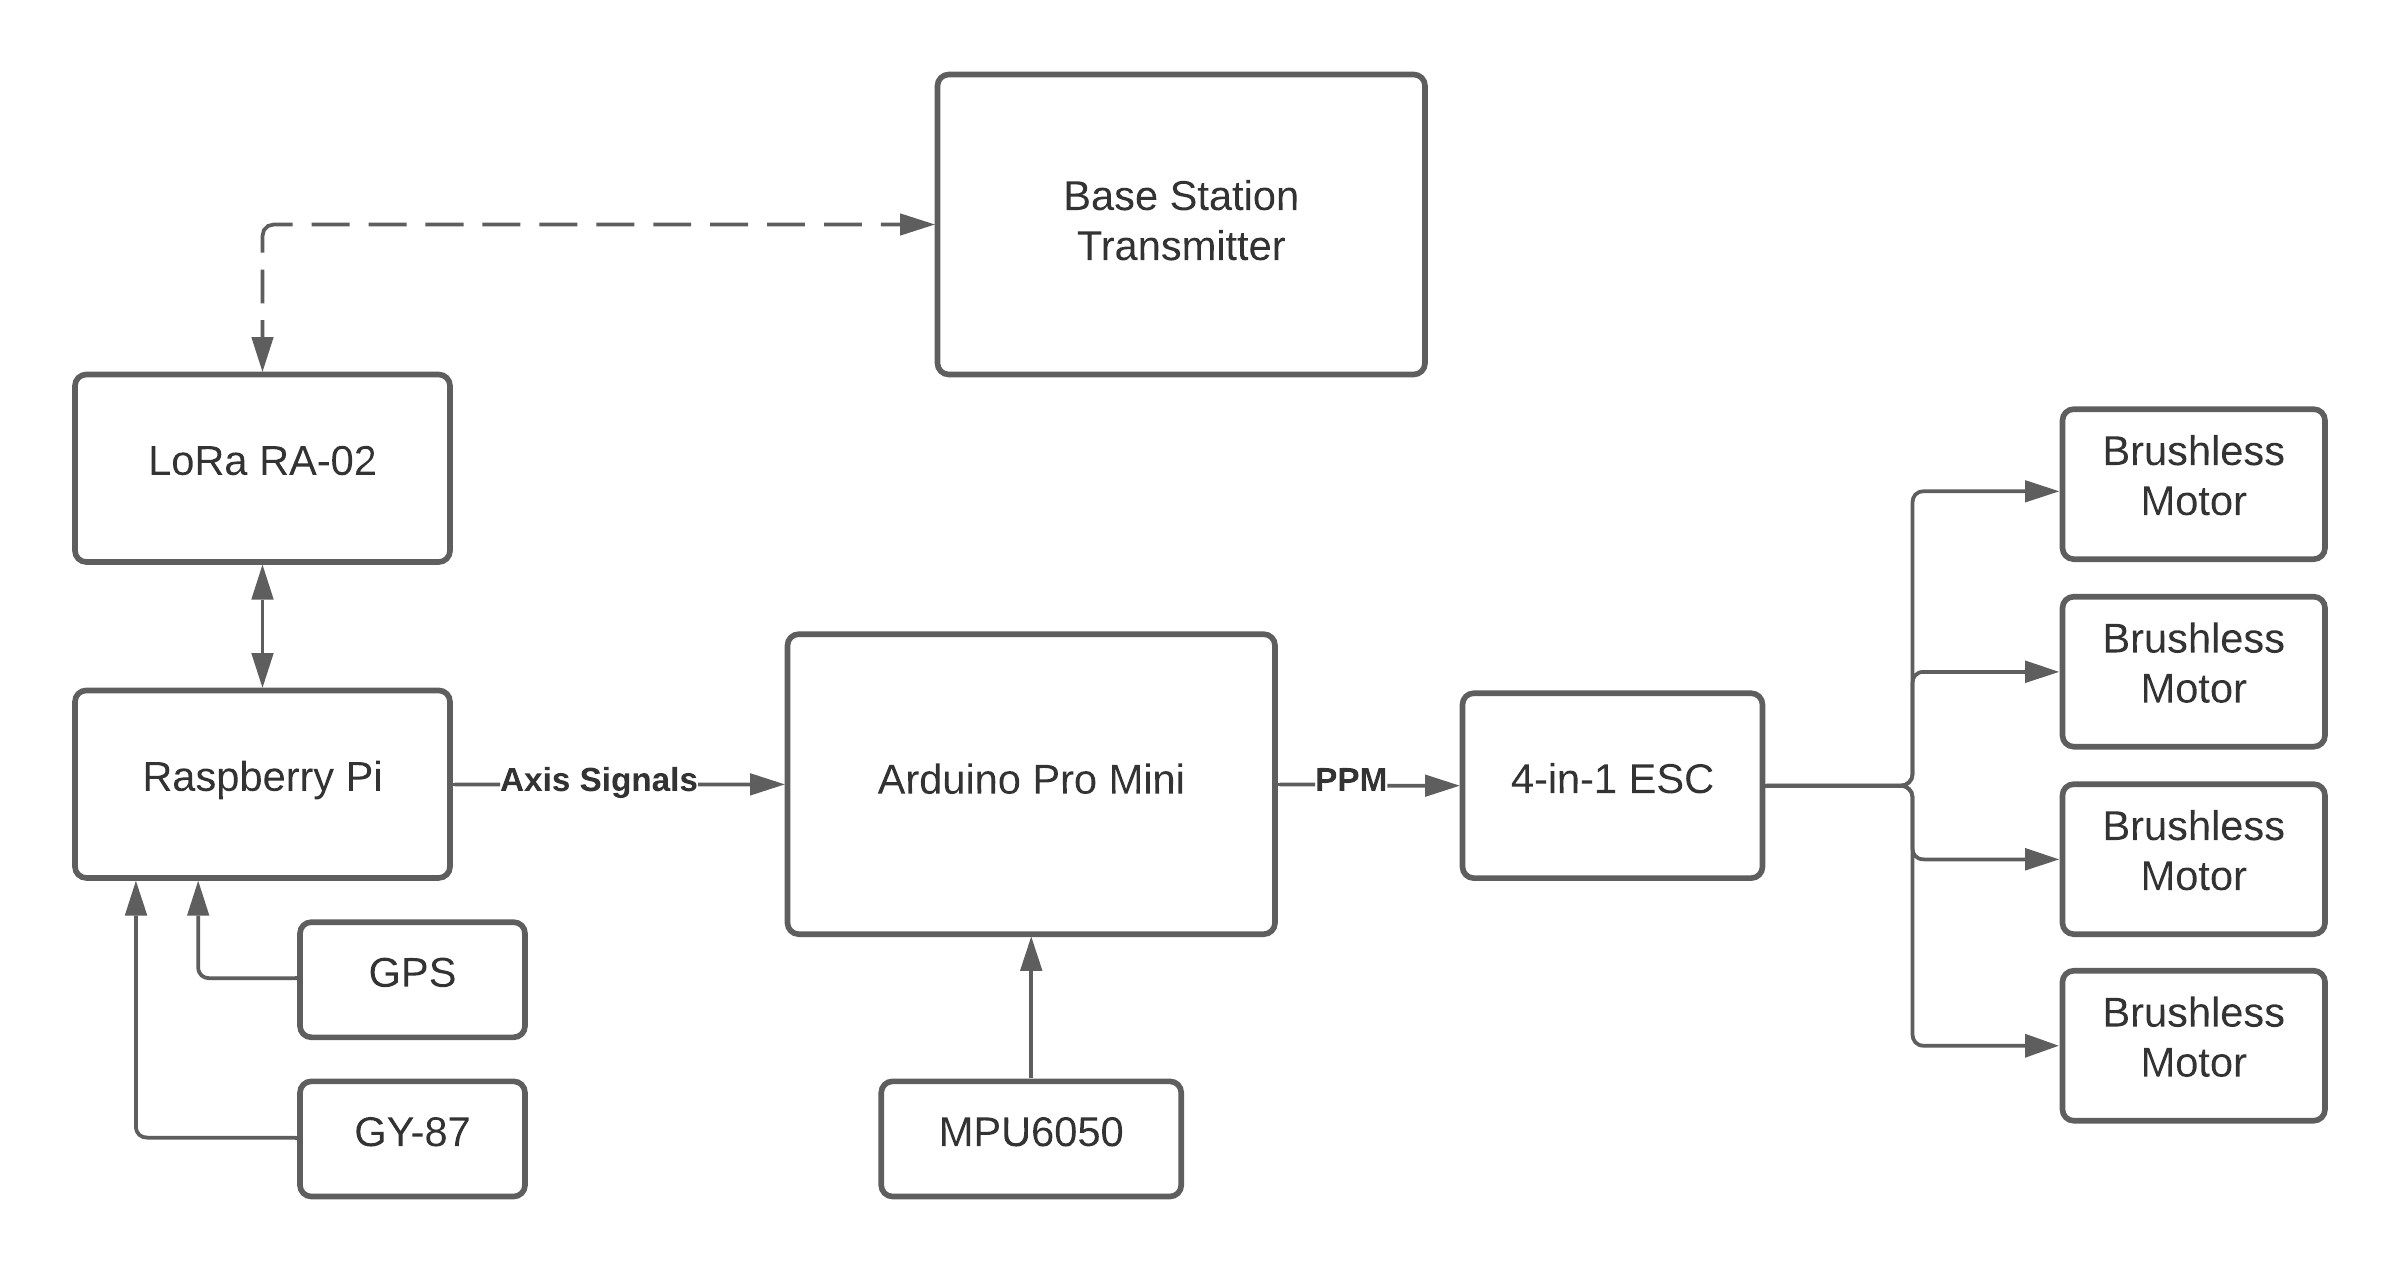
\includegraphics[scale=0.5]{images/final_FC diagram.png}
    \caption{Flight controller diagram with ESC module and motors}
    \label{fig:final_FC_diagram}
\end{figure}
\newline
\newline
The flight controller board has already been designed and fabricated to include the necessary components. This can be seen
in figure \ref{fig:fc_board}. While quantitative tests have yet to be conducted, the flight controller has been verified to
be able to run the motors at variable speeds. Further work needs to be done in order to refine the motor control. These include
tuning and calibration, which will be done during the project proper.
\begin{figure}[h]
    \centering
    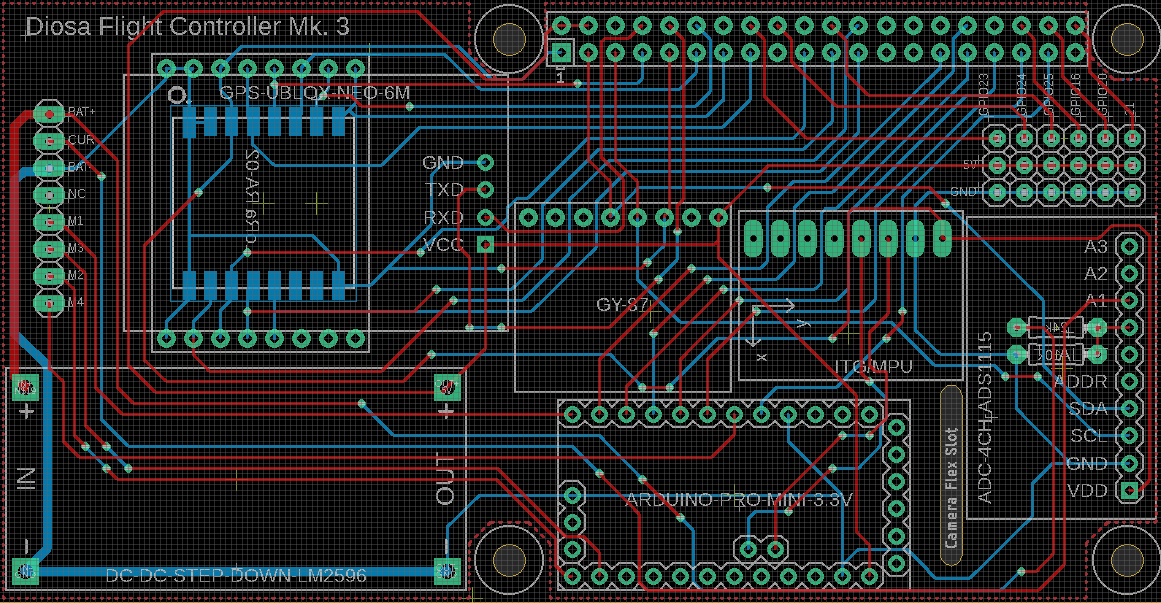
\includegraphics[scale=0.5]{images/board.PNG}
    \caption{Flight controller board}
    \label{fig:fc_board}
\end{figure} 
\newline
\newline
The Raspberry Pi is running the latest version of Raspbian. It also uses ROS (robot operating system) for
the UAV's processes. ROS is an open source robotics framework that was designed to be modular and flexible, taking into
account the multitude of processes that a robot needs to run. In the case of this project, the modularity allows for
easier integration of different modules and functions. This in turn means that the source code will be easier to maintain
as more and more functions are added.
\chapter{Methodology}
This project can be divided into three milestones; flight controller calibration, integration of SLAM, and
finally, integration of autonomous navigation system.
\section{Flight Controller Tuning and Calibration}
With the flight controller fabricated, it then needs to be calibrated and tuned. Fortunately, the MultiWii also
comes with a GUI that allows users to calibrate and tune the sensors and PID values. The gyroscope and accelerometer may
be calibrated automatically via the GUI however the PID values must be calibrated manually. Typical heuristic methods
involve test flights where a pilot performs sharp maneuvers in order to see how the UAV reacts. They then come back to the
interface and adjust the PID values based on trial and error. After calibration and tuning, the UAV should function 
similarly to an off-the-shelf quadcopter.
\section{SLAM Integration}
There are two outstanding choices for SLAM; Orb SLAM 2 \cite{OrbSlam2} and SVO \cite{SVO2017}. Orb SLAM 2 provides a
powerful and fast out-of-the-box solution for SLAM however due to the processing power restrictions, SVO proves to be the
more ideal system. Luckily, the developers have already provided a means to integrate SVO into the ROS framework.
Therefore, applying SVO to the UAV should be a trivial matter. Data from SVO will then be communicated via the RA-02
module back to the base station so that the pilot may have a real-time view of how the mapping operation is progressing.
\section{Autonomous Navigation and Exploration}
Two possible systems may be chosen for autonomous Navigation; the FUEL system\cite{Fuel2020} that is built
upon the frontier method of navigation and the method that uses a probabilistic roadmap as demonstrated by Xu et al.\cite{ProbNav}.
In order to see which navigation system is the best fit, both systems will be implemented and benchmark tests will be run.
The systems will be compared in terms of exploration speed, efficiency (i.e. the tests will favor the method that generates the
shortest flight path to completely explore a region), completeness (i.e. the method must not leave any region within the
enclosed space unexplored), and ability to safely navigate around obstacles.
\chapter{Timeline}
\section{Gantt Chart}
\begin{figure}[h]
    \centering
    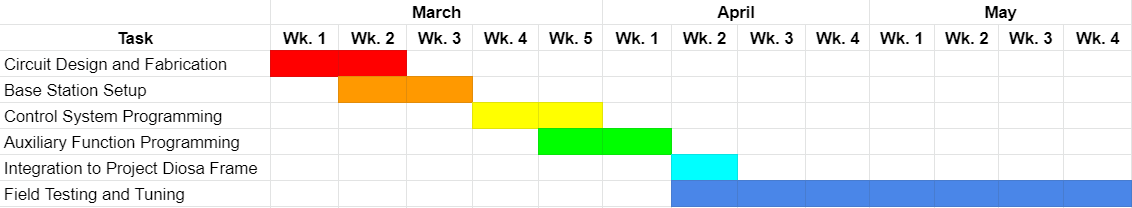
\includegraphics[scale=0.5]{images/gantt_chart.PNG}
    \caption{Project gantt chart}
    \label{fig:gantt_chart}
\end{figure}
\section{Halfway Deliverables}
By the end of March, the following deliverables should be ready:
\begin{enumerate}
    \item Flight controller achieves the following specifications:
    \begin{itemize}
        \item UAV must be able to collect inertial data from the integrated IMU
        \item GPS is able to obtain UAV's geographical coordinates and send it to the base station
        \item Capable of sending and receiving data through integrated LoRa module
        \item Should be able to perform stable non-autonomous flight at a fixed height for at least 10 minutes.
    \end{itemize}
    \item Operational SLAM system using SVO
    \begin{itemize}
        \item Should be able to perform SLAM in real-time
        \item Should be able to store map data on a global scale rather than just a local one (i.e. aside from being able
        to map out the UAV's current region, the drone must be able to store map data of other regions connected to it that
        the UAV has already explored)
        \item Should be able to transmit map data to base station
    \end{itemize}
\end{enumerate}

\section{End of Project Deliverables}
In addition to the deliverables listed above, by the end of the given time period, the project must have accomplished
the following:
\begin{enumerate}
    \item Autonomous exploration and navigation
    \begin{itemize}
        \item The UAV should be able to generate a complete map of all reqions within an enclosed space (i.e. There must be
        no unexplored regions within the enclosed space after the UAV is done exploring).
        \item The UAV should be able to autonomously navigate while flying at a speed of at least 0.5 m/s
        \item After mapping a space, the UAV should be able to safely return to the origin
    \end{itemize}
\end{enumerate}
\printbibliography[
heading=bibintoc,
title={Bibliography}
]

\end{document}

